%%%%%%%% latex template for graduate thesis
%%%%%%%% credits : I. Rigopoulos, I. Moschidou,  K. Draziotis

%%%%%%%% Licence GPL
% Ιf someone improve this template he/she can add his/her name and send it back to drazioti@gmail.com
% Compile main.tex with latex and bibtex 


\documentclass[12pt]{article}
\usepackage{helvet} 
\usepackage{mathtools}
\usepackage{amsmath}
\usepackage{titlesec}
\usepackage{lipsum}
\usepackage{textcomp}

\titleformat{\section}[display]
          {\clearpage\vspace*{50pt}%
          \normalfont\huge\bfseries}%
          {{\Kappa}E{$\Phi$}A{$\Lambda$}AIO \thesection}%
          {20pt}%
          {\Huge}%
          [\vspace{40pt}]
\usepackage[algosection,commentsnumbered,ruled,vlined]{algorithm2e}
\NoCaptionOfAlgo
\usepackage{chemarrow}
\newcommand\aug{\fboxsep=-\fboxrule\!\!\!\fbox{\strut}\!\!\!}
\usepackage{graphicx}
%\usepackage{gfsdidot}
\usepackage[LGR,T1]{fontenc}
\usepackage[utf8]{inputenc}
\usepackage[english,greek]{babel} % και για τις δυο γλώσσες
\usepackage{alphabeta}
\usepackage[hidelinks]{hyperref}
\usepackage{hyperref}
\usepackage{makeidx}
\usepackage{enumerate}
\usepackage{enumitem}
\usepackage{systeme}
\usepackage{algorithmic}
%\usepackage[linesnumbered,ruled,vlined]{algorithm2e}
\usepackage{geometry}
\usepackage{float}
\geometry{
 a4paper,
 %total={170mm,257mm},
 left=25mm,
 right=25mm,
 %top=20mm,
 }
 
 %% το παρακάτω χρησιμοποιείται για την εισαγωγή κώδικα
\usepackage{listings}
 \usepackage{xcolor}
\definecolor{codegreen}{rgb}{0,0.6,0}
\definecolor{codegray}{rgb}{0.5,0.5,0.5}
\definecolor{codepurple}{rgb}{0.58,0,0.82}
\definecolor{backcolour}{rgb}{0.95,0.95,0.92}
\lstdefinestyle{mystyle}{
    backgroundcolor=\color{backcolour},   
    commentstyle=\color{codegreen},
    keywordstyle=\color{magenta},
    numberstyle=\tiny\color{codegray},
    stringstyle=\color{codepurple},
    basicstyle=\ttfamily\footnotesize,
    breakatwhitespace=false,         
    breaklines=true,                 
    captionpos=b,                    
    keepspaces=true,                 
    numbers=left,                    
    numbersep=5pt,                  
    showspaces=false,                
    showstringspaces=false,
    showtabs=false,                  
    tabsize=2,
    upquote=true,
    columns=fullflexible
}
\lstset{style=mystyle}

\newtheorem{algor}{\bf{Αλγόριθμος}}[subsection]
\newcommand{\lt}{\latintext}

\def\tl{\textlatin }

\begin{document}

%%%%%%%%%%%%%%%%%%%%%%% PAGE 0 %%%%%%%%%%%%%%%%%%%%%%%%%%%%%
\pagenumbering{gobble} %no numbering

\begin{figure}[h] %top of the page
\vspace*{-1cm}
\centering

\includegraphics[scale=0.35]{pictures/AUThLogo.png}
\end{figure}

%{\Large  \centering {ΑΡΙΣΤΟΤΕΛΕΙΟ ΠΑΝΕΠΙΣΤΙΜΙΟ ΘΕΣΣΑΛΟΝΙΚΗΣ}}
%\maketitle
\begin{center}
 { \large \bf ΑΡΙΣΤΟΤΕΛΕΙΟ ΠΑΝΕΠΙΣΤΗΜΙΟ ΘΕΣΣΑΛΟΝΙΚΗΣ
  \\ ΣΧΟΛΗ ΘΕΤΙΚΩΝ ΕΠΙΣΤΗΜΩΝ 
   \\ΤΜΗΜΑ ΠΛΗΡΟΦΟΡΙΚΗΣ
    \\}
\vspace{2cm}

{\large \bf Ο ΑΛΓΟΡΙΘΜΟΣ ΤΗΣ ΑΠΟΙΚΙΑΣ ΜΥΡΜΗΓΚΙΩΝ ΚΑΙ ΕΦΑΡΜΟΓΕΣ}
    
\vspace{2.5cm}

{\large \bf ΠΤΥΧΙΑΚΗ ΕΡΓΑΣΙΑ
\\ \lt{ΜΠΙΚΑΣ ΕΥΑΓΓΕΛΟΣ}
  \\2947}
  
  \vspace{2cm}
  
  {\sc{ΕΠΙΒΛΕΠΩΝ: \lt{Κ.ΔΡΑΖΙΩΤΗΣ}}}
\end{center}


\newpage
{\latintext

\begin{figure}[h] %top of the page
\vspace*{-1cm}
\centering

\includegraphics[scale=0.35]{pictures/AUThLogo.png}
\end{figure}

\begin{center}
 { \large \bf ARISTOTLE UNIVERSITY OF THESSALONIKI
  \\ SCHOOL OF EXACT SCIENCES 
   \\COMPUTER SCIENCE DEPARTMENT
    \\}
\vspace{2cm}

{\large \bf THE ANT COLONY ALGORITHM AND APPLICATIONS}
    
\vspace{2.5cm}

{\large \bf GRADUATE THESIS
\\ \lt{BIKAS EVANGELOS}
  \\2947}
  
  \vspace{2cm}
  
  {\sc{SUPERVISOR: \lt{K.DRAZIOTIS}}}
\end{center}

%%%%%%%%%%%%%%%%%%%%%%%%% PAGE 1 %%%%%%%%%%%%%%%%%%%%%%%%%%%

\newpage
\pagenumbering{arabic} %get the Numbers back

\begin{minipage}{0.12\textwidth}
	    
\includegraphics[width=\linewidth]{pictures/AUThLogo.png}
	\end{minipage}
	\hspace{1em}
	\begin{minipage}{0.65\textwidth}
    	Αριστοτέλειο Πανεπιστήμιο Θεσσαλονίκης\\
    	Σχολή Θετικών Επιστημών \\
    	Τμήμα Πληροφορικής
	\end{minipage}


\vspace{2.5cm}
{\bf \lt Copyright \textcopyright  All rights reserved} {\bf \lt{Μπίκας Ευάγγελος}, 2022.}
\\
\vspace{0.5cm}
\\
{ Με πλήρη επίγνωση των συνεπειών του νόμου περί πνευματικών δικαιωμάτων, δηλώνω ρητά ότι η παρούσα πτυχιακή εργασία, καθώς και τα ηλεκτρονικά αρχεία και πηγαίοι κώδικες που αναπτύχθηκαν ή τροποποιήθηκαν στο πλαίσιο αυτής της εργασίας, αποτελεί αποκλειστικά προϊόν προσωπικής μου εργασίας, δεν προσβάλλει κάθε μορφής δικαιώματα διανοητικής ιδιοκτησίας, προσωπικότητας και προσωπικών δεδομένων τρίτων, δεν περιέχει έργα/εισφορές τρίτων για τα οποία απαιτείται άδεια των δημιουργών/δικαιούχων και δεν είναι προϊόν μερικής ή ολικής αντιγραφής, οι πηγές δε που χρησιμοποιήθηκαν περιορίζονται στις βιβλιογραφικές αναφορές και μόνον και πληρούν τους κανόνες της επιστημονικής παράθεσης. Τα σημεία όπου έχω χρησιμοποιήσει ιδέες, κείμενο, αρχεία ή/και πηγές άλλων συγγραφέων, αναφέρονται ευδιάκριτα στο κείμενο με την κατάλληλη παραπομπή και η σχετική αναφορά περιλαμβάνεται στο τμήμα των βιβλιογραφικών αναφορών με πλήρη περιγραφή. Αναλαμβάνω πλήρως, ατομικά και προσωπικά, όλες τις νομικές και διοικητικές συνέπειες που δύναται να προκύψουν στην περίπτωση κατά την οποία αποδειχθεί, διαχρονικά, ότι η εργασία αυτή ή τμήμα της δεν μου ανήκει διότι είναι προϊόν λογοκλοπής.}
\\
\vspace{0.5cm}
\\
{ Το περιεχόμενο αυτής της εργασίας δεν απηχεί απαραίτητα τις απόψεις του Τμήματος, του
Επιβλέποντα, ή της επιτροπής που την ενέκρινε.}
\\
\vspace{0.5cm}
\\
\\
{\bfseries Υπεύθυνη Δήλωση}
\\ \\
{\bfseries (Υπογραφή)}
......................................
\ \\\\
{ \bfseries {\lt{Μπίκας Ευάγγελος}}}

%%%%%%%%%%%%%%%%%%%%%% PAGE 2-3 %%%%%%%%%%%%%%%%%%%%%%%%%%

\newpage
%Abstract/Περιγραφή
\begin{abstract}
 Σκοπός της παρούσας πτυχιακής εργασίας είναι η παρουσίαση και υλοποίηση του αλγόριθμου της αποικίας των μυρμηγκιών. Ο αλγόριθμος αυτός είναι ένας αλγόριθμος βελτιστοποίησης που είναι βασισμένος σε παρατηρήσεις που έγιναν στα μυρμήγκια στην φύση. Πιο συγκεκριμένα, έχει μελετηθεί ο τρόπος με τον οποίο καταφέρνουν να αλληλεπιδρούν μεταξύ τους και το πως βρίσκουν πάντα την βέλτιστη διαδρομή από την φωλιά τους μέχρι την πηγή τροφής. 

 Αυτό το πετυχαίνουν εκπέμπτοντας χημικές ουσίες που τις χρησιμοποιούν ως σήματα επικοινωνίας, τις λεγόμενες φερομόνες. Ο αλγόριθμος που θα αναλύσουμε είναι μία προσομοίωση αυτής της συμπεριφοράς με χρήση τεχνητών μυρμηγκιών.
 
Το γεγονός ότι βρίσκει βέλτιστη λύση σε συνδυασμό με το πόσο γρήγορα επιτυγχάνεται και το ότι μπορούν να εφαρμοστούν πολλές παραλλαγές του ανάλογα με το ζητούμενο καθιστά αυτόν τον αλγόριθμο χρήσιμο σε διάφορους τομείς, όπως η επεξεργασία εικόνων και οι τηλεπικοινωνίες. Εντάσεται σε πολλά πεδία και εφαρμογές που έχουν ως στόχο την βελτιστοποίηση, με κλασικό παράδειγμα αυτό του πλανόδιου πωλητή.

Παρακάτω, θα αναλυθεί η θεωρία γράφων και το πως σχετίζεται με αλγόριθμους βελτιστοποίησης, θα αναφερθούν κάποιοι αλγόριθμοι βελτιστοποίησης με έμφαση στον αλγόριθμο της αποικίας των μυρμηγκιών. Θα παρουσιαστεί η δική μου υλοποίηση, θα συγκριθεί με παραλλαγές αυτού και άλλων αλγοριθμων βελτιστοποίησης και θα δωθούν πιθανές εφαρμογές σε προβλήματα πραγματικόύ κόσμου σε τομείς όπως η επιστήμη των υπολογιστών. Όλοι οι αλγόριθμοι θα υλοποιηθούν σε python.

{\bf Λέξεις Κλειδιά}.
    Προβλήματα Βελτιστοποίησης,  Αλγόριθμος Αποικίας Μυρμηγκιών, Θεωρία Γράγων {\lt, Python} 
\end{abstract}    
\newpage
{\latintext
\begin{center}
{\sc{summary}}
\end{center}
{\small
	{\lt The purpose of this thesis is the presentation and implementation of the ant colony algorithm. This algorithm is an optimization algorithm that is based on observations made on ants in nature. More specifically, the way in which they manage to interact with each other and how they always find the optimal route from their nest to the food source has been studied.

  They achieve this by emitting chemicals that they use as communication signals, so-called pheromones. The algorithm we will analyze is a simulation of this behavior using artificial ants.
 
 The fact that it finds an optimal solution combined with how fast it is achieved and that many variations of it can be applied depending on the application make this algorithm useful in various fields such as image processing and telecommunications, and span many fields and applications. which aim at optimization, with the classic example of that of the traveling salesman.

Below we will discuss graph theory and how it relates to optimization algorithms, introduce some optimization algorithms with an emphasis on the ant colony algorithm, present my own implementation and compare it to variations of this and other optimization algorithms, and give possible applications in real-world problems in fields such as computer science. All algorithms will be implemented in python.}
	\ \\\\
{\bf Key Words.} Οptimization Problems, Ant Colony Algorithm, Graph Theory, Python
}}

%%%%%%%%%%%%%%%%%%%%%% PAGE 4 %%%%%%%%%%%%%%%%%%%%%%%%%%
\newpage

% Πίνακας Περιεχομένων
\tableofcontents

\newpage

%%%%%%%%%%%%%%%%%%%%%%%%%%%%%%%%%%%%%%%%%%%%%%%%%%%%%
%% INCLUDE YOUR CHAPTERS/SECTIONS HERE
%%
%\mainmatter

%Εισαγωγή
\section{Εισαγωγή}
\selectlanguage{greek}
Ένα μεμονωμένο μυρμήγκι δεν μπορεί να κάνει πολλά, τα μυρμήγκια ως σύνολο όμως, όπως και κάθε άλλο είδος εντόμων που λειτουργούν ομαδικά ως σμήνος για την επίτευξη κοινού στόχου, μπορούν να ολοκληρώσουν εξειδικευμένες εργασίες γρήγορα και αποτελεσματικά. Αυτό αποτελεί πηγή έμπνευσης για τον αλγόριθμο που θα μελετήσουμε σε αυτήν την εργασία καθώς και για πολλούς άλλους αλγόριθμους σμήνους που έχουν ως στόχο την επίλυση πολύπλοκων προβλημάτων βελτιστοποίησης πραγματικού κόσμου \cite{dorigo2004ant}. 

Τα τελευταία χρόνια, τέτοια προβλήματα παρουσιάζονται σε διάφορους κλάδους με πλη- θώρα θεωρητικών και πρακτικών εφαρμογών όπως το πρόβλημα γεφυρών και το πρόβλημα του πλανόδιου πωλητή (\lt{Travelling Salesman Problem - TSP}) καθώς και σε κοινωνικά δίκτυα, δίκτυα δρομολόγησης \cite{gkertsis2023thewria}, προβλήματα προσβασιμότητας, βελτιστοποίηση δικτύων επικοινωνίας, σχεδίαση ηλεκτρικών κυκλωμάτων, και άλλα, για το λόγο αυτό, ιδιαίτερο ε- νδιαφέρον έχει αναπτυχθεί για την μελέτη τους \cite{manwlopoulos2014thewria}.

Ο αλγόριθμος της αποικίας μυρμηγκιών (\lt{Ant Colony Optimisation - ACO}) που θα αναλυθεί στην παρούσα πτυχιακή εργασία είναι ένας αλγόριθμος νοημοσύνης σμήνους και με χρήση αυτού αντιμετωπίζονται τέτοια προβλήματα. Ο όρος "Νοημοσύνη Σμήνους" (\lt{swarm intelligence}) πρωτοεμφανίστηκε το 1989 από τους \lt{Gerardo Beni} και \lt{Jing Wang} \cite{10.1007/978-3-642-58069-7_38} και μας βοηθάνε στην επίλυση προβλημάτων βελτιστοποίησης, ενώ το 1992 προτάθηκε ο \lt{ACO} μέσω της διδακτορικής διατριβής του \lt{Marco Dorigo}. Οι αλγόριθμοι αυτοί μιμούνται εξελικτικές διαδικασίες που παρουσιάζονται στην φύση όπως η επιλογή μιας διαδρομής και η προσαρμογή σε νέα δεδομένα. Ο αλγόριθμος της αποικίας των μυρμηγκιών συγκεκριμένα βασίζεται, όπως προκύπτει κι από το όνομα του, στη συμπεριφορά των μυρμηγκιών στην φύση και το πώς καταφέρνουν πάντα να βρίσκουν την βέλτιστη διαδρομή σε όποιο πρόβλημα τους παρουσιαστεί με χρήση πιθανολογικών τεχνικών. Πέρα από τον \lt{ACO}, παραδείγματα άλλων τέτοιων αλγορίθμων είναι ο αλγόριθμος βελτιστοποίησης σμήνους σωματιδίων (\lt{Particle Swarm Optimisation - PSO}), ο αλγόριθμος των μελισσών (\lt{Artificial Bee Colony Algorithm - ABC}), οι διάφοροι γενετικοί αλγόριθμοι (\lt{Genetic Algorithms- GA}) και πολλοί άλλοι \cite{mavrovouniotis2017survey}.

Ένα κεφάλαιο απαραίτητο για την υλοποίηση αυτού του αλγόριθμου είναι η θεωρία γράφων. Έννοιες στις οποίες βασίζεται ο \lt{ACO} όπως η φερομόνη (\lt{pheromone}) και το κόστος διαδρομής (\lt{cost}), μοντελοποιούνται με χρήση αυτής. Κάθε ακμή (\lt{edge}) του γράφου αντιστοιχεί σε μία τιμή φερομόνης, η οποία ανανεώνεται καθώς τα μυρμήγκια περνούν από αυτήν. Τα μυρμήγκια εξερευνούν πιθανές διαδρομές, και ενισχύουν την ποσότητα φερομόνης στις καλύτερες, επηρεάζοντας έτσι τις επιλογές των μυρμηγκιών που ακολουθούν δίνοντας στον αλγόριθμο την δυνατότητα να "θυμάται" προηγούμενες λύσεις και να τις αξιοποιεί στο μέλλον. 


\begin{flushright} 
    \lt{I am lost! Where is the line?!
    
    —A Bug’s Life, Walt Disney, 1998}\cite{dorigo2004ant}
\end{flushright}

\subsection{Ιστορική Αναδρομή}
\begin{figure}[ht]
    \begin{minipage}[c]{.46\linewidth}
        \centering
        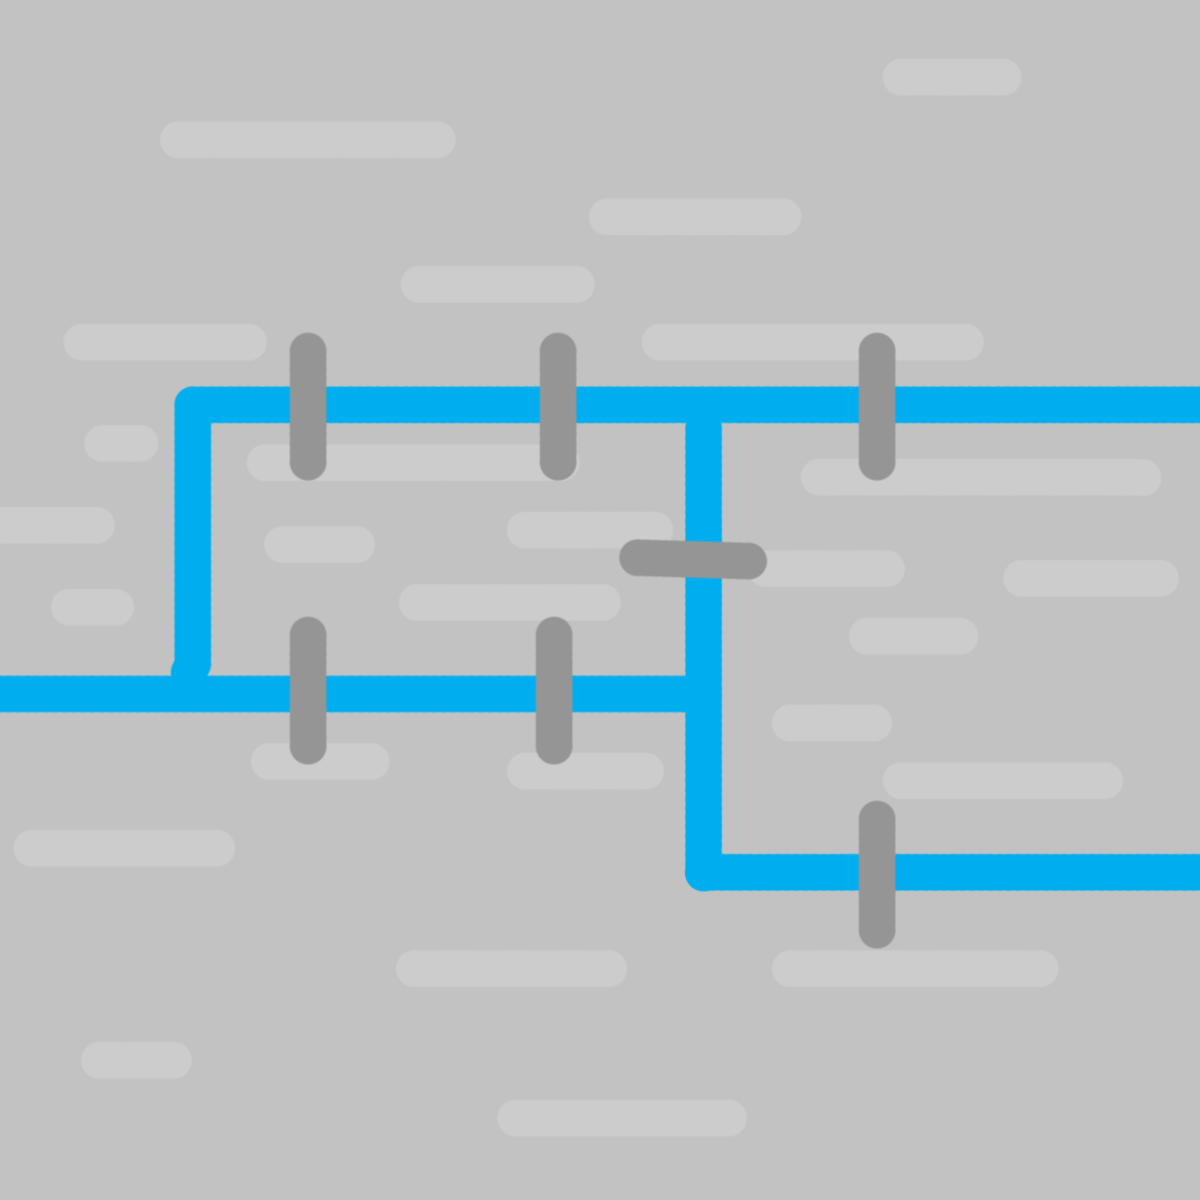
\includegraphics[scale=0.15]{2947_thesis/pictures/konigsberg.png}
        \caption{Προσομοίωση Königsberg.}
        \label{1}
    \end{minipage}
    \hfill%
    \begin{minipage}[c]{.46\linewidth}
        \centering
        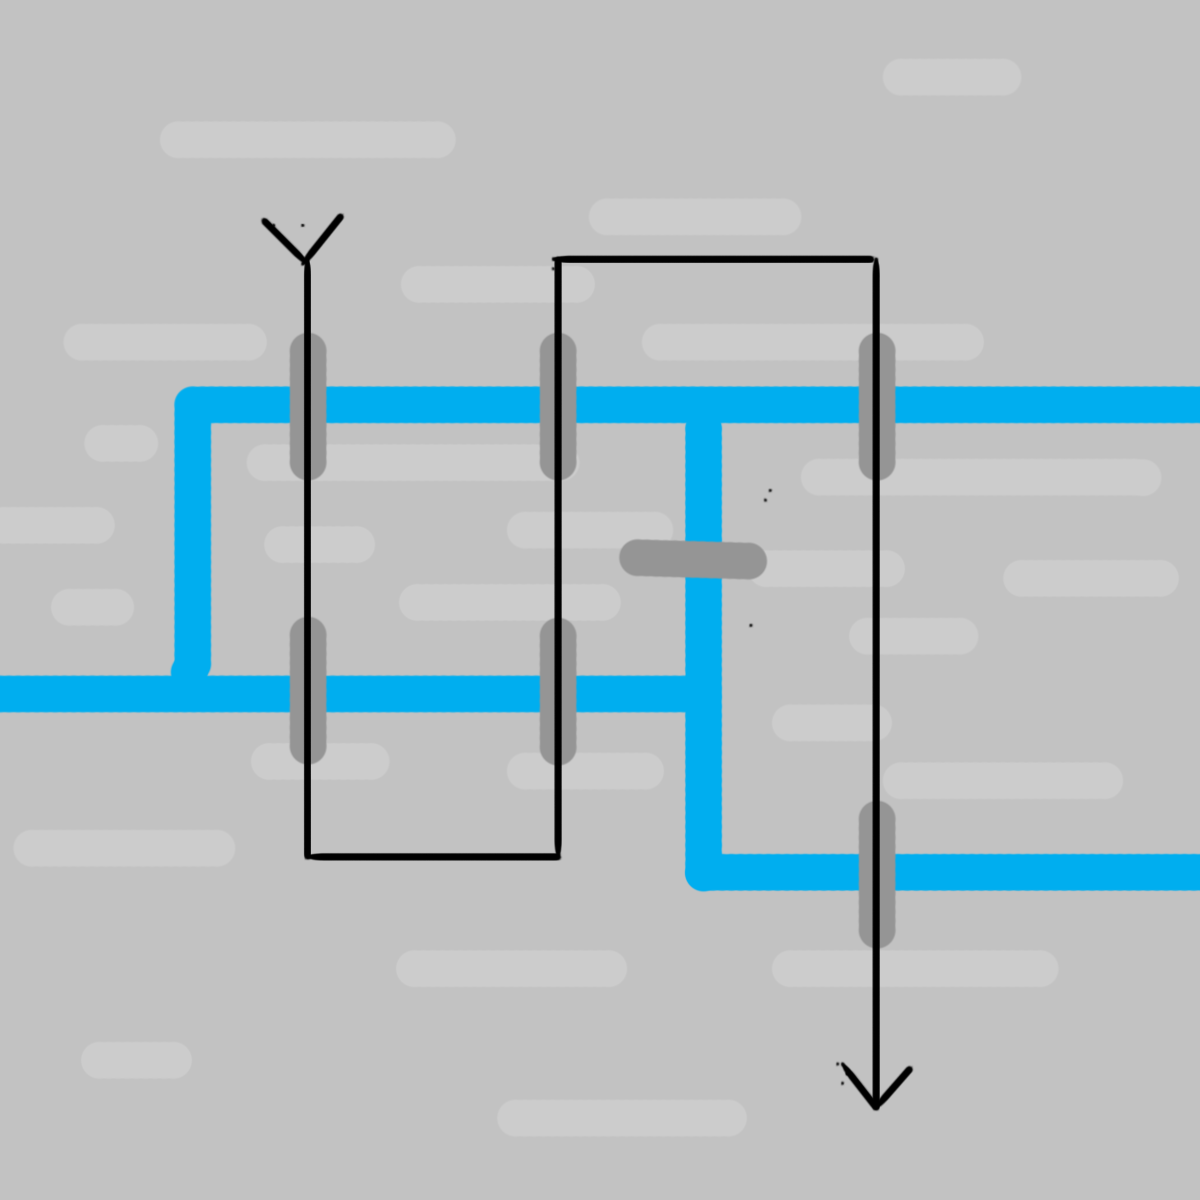
\includegraphics[scale=0.15]{2947_thesis/pictures/konigsbergEx.png} 
        \caption{Παράδειγμα διάσχισης γεφυρών}
        \label{2}
    \end{minipage}
\end{figure}
Η ανάπτυξη της θεωρίας γράφων (\lt{graph theory}) ξεκίνησε τον 18ο αιώνα και πιο συγκεκριμένα το 1736 στην πόλη \lt{Königsberg} της Πρωσίας. Σήμερα είναι το Ρωσικό \lt{Kaliningrad} (μεταξύ Λιθουανίας και Πολωνίας στη Βαλτική) \cite{manwlopoulos2014thewria}. Η πόλη ήταν χωρισμένη σε 4 τμήματα από τον ποταμό \lt{Pregel} και χρησιμοποιούνταν 7 γέφυρες για να γίνεται εφικτή η διέλευση των κατοίκων στα διάφορα τμήματά της εικόνας \ref{1}. Όταν ο Ελβετός μαθηματικός \lt{Leonard Euler} αναρωτήθηκε αν είναι εφικτό να διασχίσει κάποιος τις γέφυρες της πόλης με βασικό περιορισμό να διασχιστούν όλες οι γέφυρες μόνο μία φορά (Πρόβλημα των 7 γεφυρών του \lt{Königsberg}) \ref{2}, ένας νέος κλάδος των διακριτών μαθηματικών γεννήθηκε, γνωστός και ως θεωρία γράφων. Ο \lt{Euler} απέδειξε ότι δεν υπάρχει τέτοια διαδρομή μέσω της χρήσης γράφων \lt{Graph Theory} και κατά συνέπεια το πρόβλημα δεν έχει λύση. Αυτή η απόδειξη απέκτησε αξία όταν ο \lt{Euler} την εφάρμοσε και σε άλλα προβλήματα γράφων και γενίκευσε την βασική ιδέα. 

Ένα μονοπάτι (\lt{path}) ονομάζεται μονοπάτι \lt{Euler (Eulerian path} ή \lt{Eulerian trail}) όταν μπορούμε να επισκεφτούμε κάθε περιοχή-κορυφή (\lt{vertice}) διασχίζοντας την κάθε γέφυρα-ακμή (\lt{edge}) μόνο μία φορά (και ονομάζεται κυκλική αν καταλήγουμε εκεί που ξεκινήσαμε), αν υπάρχει ένα τέτοιο μονοπάτι σε ένα γράφο τότε αυτός ο γράφος ονομάζεται γράφος \lt{Euler} (\lt{Eulerian graph}) \cite{ntenisiwtis2023thewria}. Στο σχήμα \ref{3} που αντιπροσωπεύει την πόλη του \lt{Königsberg} σε μορφή γράφου δεν υπάρχει μια τέτοια διαδρομή. Για να γίνει αυτό πρέπει να αφαιρέσουμε μία γέφυρα-ακμή όπως φαίνεται στο σσχήμα \ref{4}. Αποδείχθηκε από τον \lt{Euler} ότι όλες οι κορυφές πρέπει να έχουν άρτιο πλήθος ακμών που προσπίπτουν σε αυτή την κορυφή (βαθμό - \lt{degree}), εκτός από αυτές  που ξεκινά και τελειώνει η διαδρομή, εκτός κι αν η διαδρομή είναι κυκλική. Πιο συγκεκριμένα, ένας συνδεδεμένος γράφος $Graph(Vertices,Edges)$ είναι γράφος Euler αν και μόνο αν δεν έχει κορυφές (\lt{vertices}) περιττού βαθμού \cite{bondy1976usr}.

%Gauss Elimination
\section{Θεωρία Γράφων}
\selectlanguage{english}

\begin{figure}[ht]
    \begin{minipage}[c]{.46\linewidth}
        \centering
        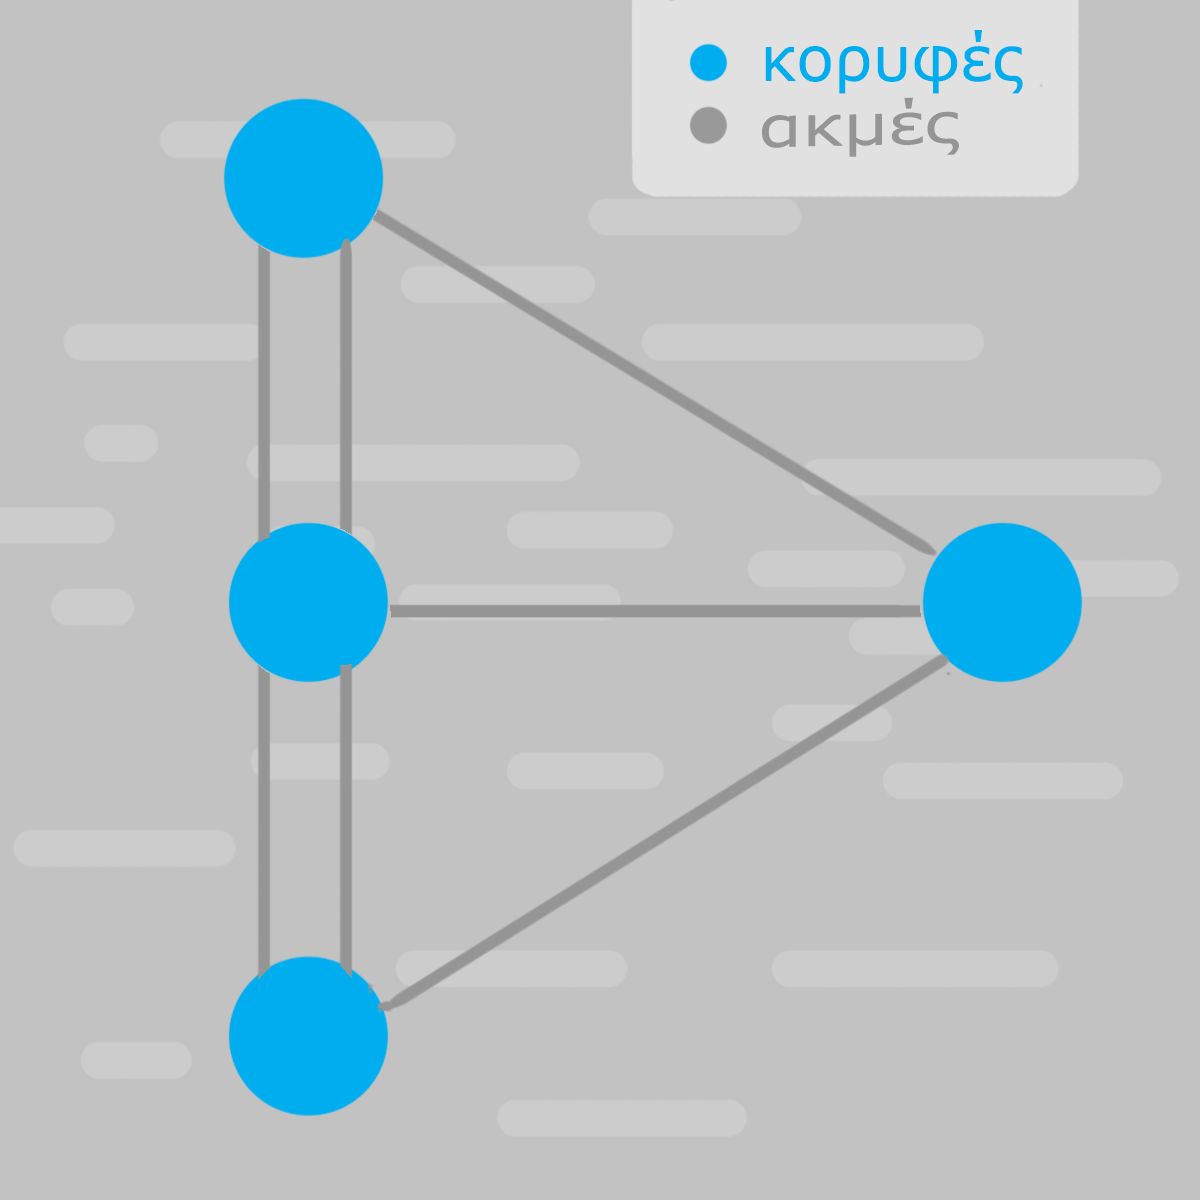
\includegraphics[scale=0.15]{2947_thesis/pictures/konigsberGraph.png}
        \caption{\lt{Königsberg} ως γράφος.}
        \label{3}
    \end{minipage}
    \hfill%
    \begin{minipage}[c]{.46\linewidth}
        \centering
        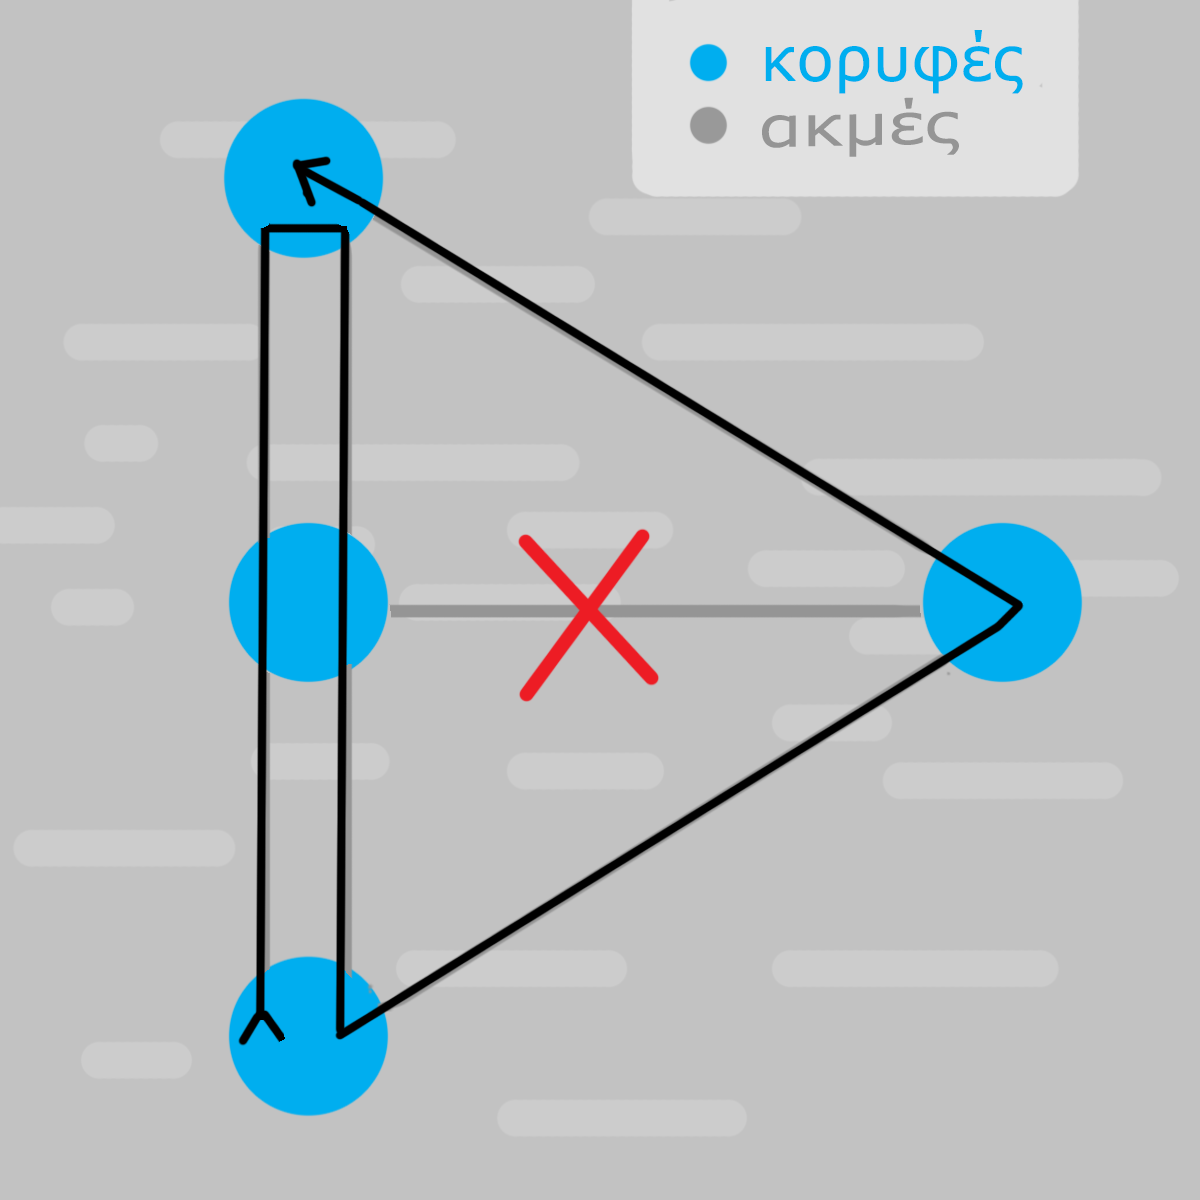
\includegraphics[scale=0.15]{2947_thesis/pictures/konigsbergEuler.png}
        \caption{Διαδρομή \lt{Euler}.}
        \label{4}
    \end{minipage}
\end{figure} 


\subsection{Εισαγωγή στην Θεωρία Γράφων}

Στην ουσία, ένας γράφος (\lt{graph}) είναι διάσπαρτα σημεία-κορυφές (\lt{vertices}) που ενώνονται με γραμμές-ακμές (\lt{edges}). Γράφους μπορούμε να συναντήσουμε σε διάφορα προβλήματα της καθημερινότητας όπως δίκτυα υποδομών (δίκτυο ύδρευσης), προβλήματα χαρτογράφησης (πλοήγηση), τηλεπικοινωνιών (δορυφόροι), μεταφορών (σιδηρόδρομοι), και άλλα \cite{manwlopoulos2014thewria}. Η θεωρία γράφων είναι ένας σημαντικός τομέας των μαθηματικών γιατί πέρα από το γεγονός ότι με χρήση αυτής μπορούμε να μοντελοποιήσουμε εύκολα προβλήματα της καθημερινότητας μας σε τομείς που αναφέρθηκαν παραπάνω, μπορούμε επίσης να αναπτύξουμε αλγόριθμους που λύνουν προβλήματα με χρήση γράφων. Παράδειγμα αυτού είναι και ο αλγόριθμος της αποικίας των μυρμηγκιών (\lt{Ant Colony Algorithm - ACO}) που θα αναλύσουμε σε αυτήν την πτυχιακή εργασία.

\subsection{Βασικοί Ορισμοί και έννοιες}
Για να γίνουν κατανοητά όσα θα αναφερθούν στην εργασία μας είναι απαραίτητο να παρουσιαστεί το θεωρητικό υπόβαθρο πάνω στο οποίο είναι βασισμένοι οι αλγόριθμοι βελτιστοποίησης. Για πιο αναλυτική μελέτη παραπέμπονται οι βιβλιογραφικές αναφορές που χρησιμοποιήθηκαν στο τέλος της εργασίας \cite{bondy1976usr}, \cite{perez2020introduction}, \cite{Gewrgiadis2017thewria}, \cite{gkertsis2023thewria}, \cite{mavrovouniotis2014ant}, \cite{ntenisiwtis2023thewria}.

Ένας γράφος είναι μία μαθηματική δομή που ορίζεται με αυστηρό τρόπο μέσω δύο συνόλων: το σύνολο κορυφών (ή κόμβων, \lt{vertices}) και το σύνολο ακμών (ή γραμμών, \lt{edges}) που συνδέουν ζεύγη κορυφών μεταξύ τους και χρησιμοποιείται για την αναπαρά- σταση πληροφορίας σχετικά με συνδεσμολογία \cite{ntenisiwtis2023thewria}. Όταν δύο κορυφές είναι συνδεδεμένες, δηλαδή ενώνονται με τουλάχιστον μία ακμή ονομάζονται γειτονικές (\lt{adjacent vertices}) (για παράδειγμα στο \ref{5} η κορυφή "Α" και η κορυφή "Β" είναι γειτονικές), αντίστοιχα δύο ακμές που καταλήγουν σε ίδια κορυφή ονομάζονται προσπίπτουσες (\lt{incident edges}) της κορυφής αυτής. Το πλήθος των ακμών που προσπίπτουν σε μία κορυφή ονομάζεται βαθμός (\lt{degree}) ή αξία (\lt{valency}) της κορυφής αυτής. Τάξη (\lt{order}) ενός γράφου καλούμε το πλήθος των κορυφών που έχει (για παράδειγμα στο σχήμα \ref{5} η κορυφή "Ε" είναι τέταρτου βα- θμού και ο γράφος είναι έκτης τάξης). Ένας γράφος μπορεί να είναι είτε κατευθυνόμενος (\lt{directed graph}) όταν οι ακμές έχουν κατεύθυνση από μία κορυφή προς μία άλλη \ref{6}, είτε μη-κατευθυνόμενος (\lt{undirected graph}) όταν οι ακμές δεν έχουν κατεύθυνση και μπορούν να πηγαίνουν προς οπουδήποτε μεταξύ των κόμβων \ref{5} \cite{gkertsis2023thewria} \footnote{για περαιτέρω μελέτη: \lt{Directed and Undirected Graphs} από \lt{mathworks}\\ link: \url{https://www.mathworks.com/help/matlab/math/directed-and-undirected-graphs.html}}.

Στις ακμές (\lt{edges}) ενός γράφου μπορεί να γίνει επισύναψη βάρους (\lt{weight}), το οποίο αντιπροσωπεύει το κόστος, την απόσταση ή άλλες χρήσιμες πληροφορίες που συνδέονται με τις σχέσεις μεταξύ των κορυφών \lt{vertices}. Ένας γράφος που οι ακμές του έχουν συσχετι- στεί με έναν αριθμό ονομάζονται γράφος με βάρη (\lt{weighted graph}). Τα βάρη μπορούν να χρησιμοποιηθούν για την εκτέλεση αλγορίθμων βελτιστοποίησης και την αναζήτηση των βέλτιστων μονοπατιών σε γράφο \cite{ntenisiwtis2023thewria}, \cite{gkertsis2023thewria}. Στον αλγόριθμο που θα αναλυθεί σε αυτήν την πτυχιακή εργασία τα βάρη αντιπροσωπεύουν την απόσταση (\lt{distance}) της διαδρομής ή το επίπεδο της φερομόνης (\lt{pheromone}) (θα αναλυθεί σε επόμενο κεφάλαιο).



\begin{figure}[ht]
    \begin{minipage}[c]{.46\linewidth}
        \centering
        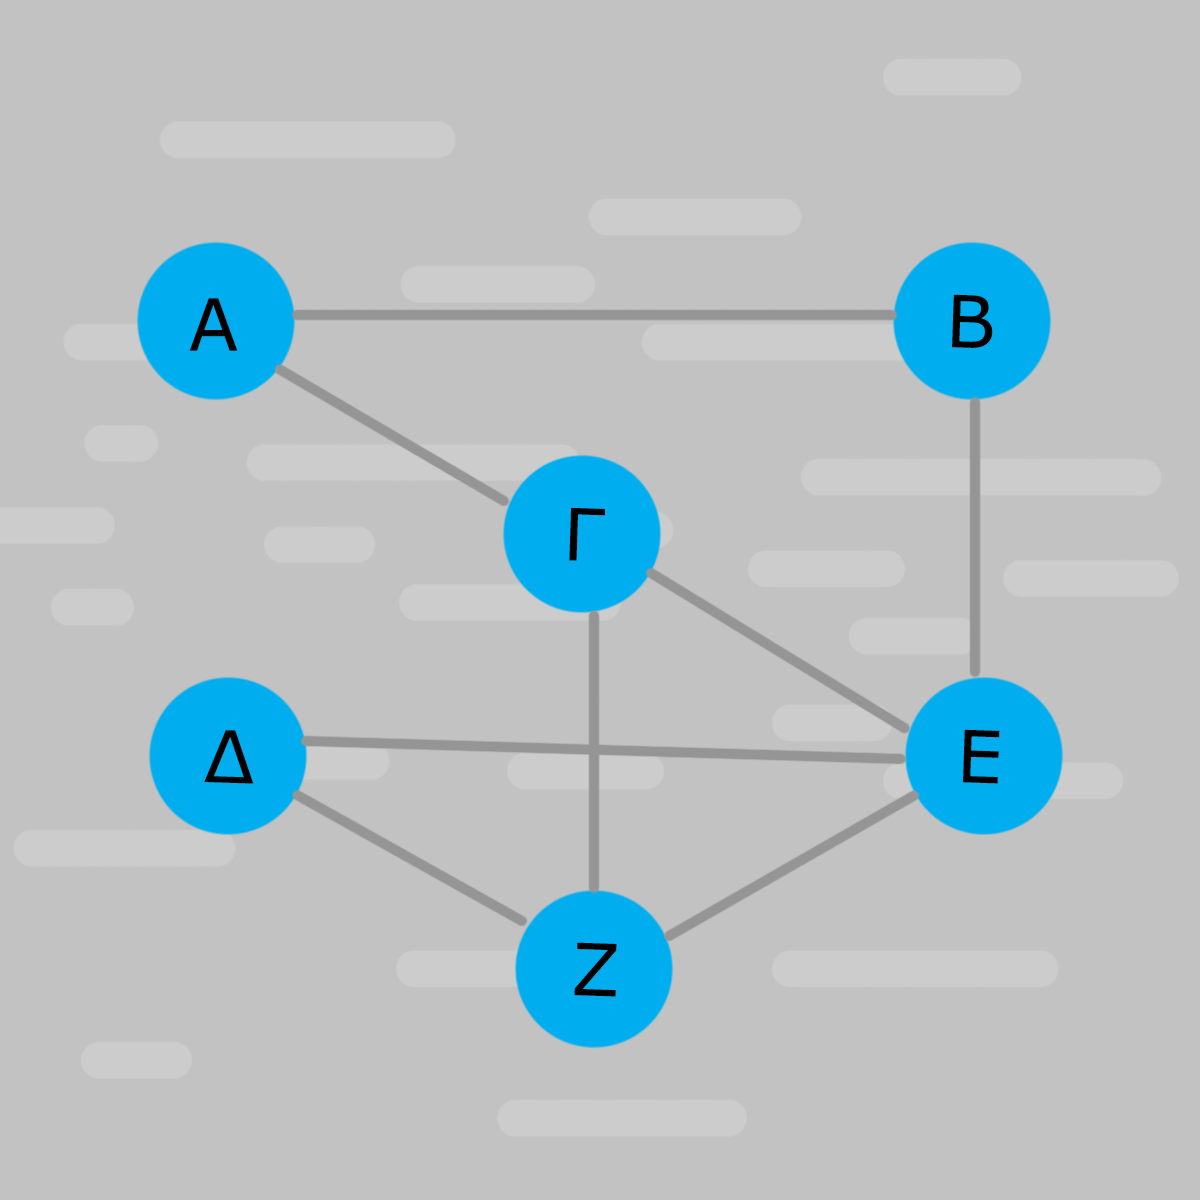
\includegraphics[scale=0.15]{2947_thesis/pictures/undirected.png}
        \caption{Μη κατευθυνόμενος γράφος.}
        \label{5}
    \end{minipage}
    \hfill%
    \begin{minipage}[c]{.46\linewidth}
        \centering
        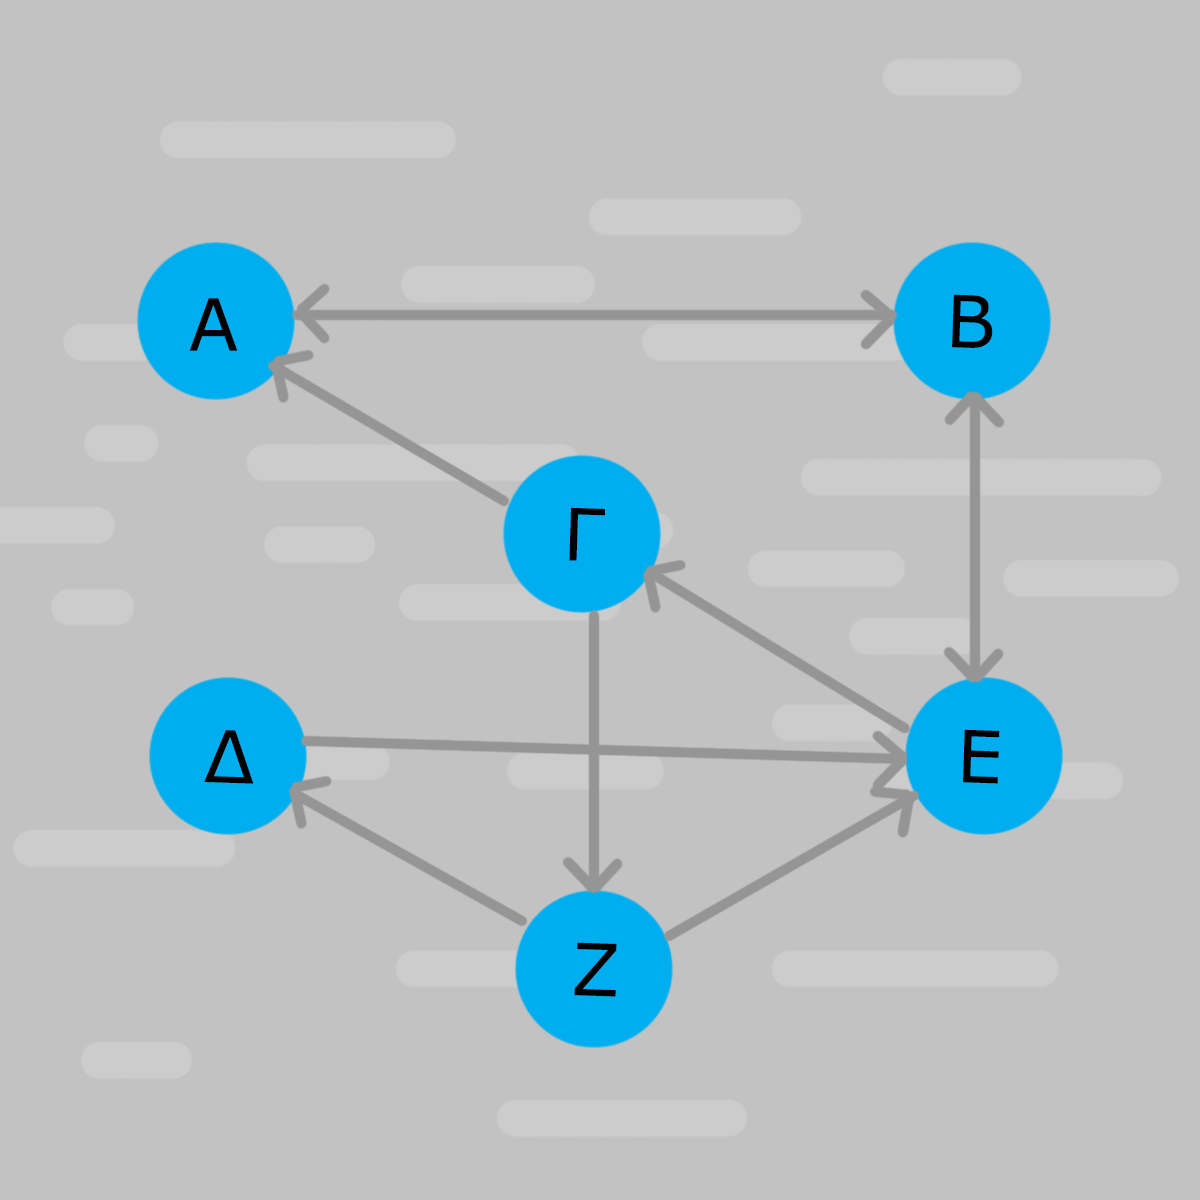
\includegraphics[scale=0.15]{2947_thesis/pictures/directed.png} 
        \caption{Κατευθυνόμενος γράφος.}
        \label{6}
    \end{minipage}
\end{figure}

\subsection{Μαθηματικό υπόβαθρο}
Ένας γράφος (\lt{Graph}) $G$ ορίζεται από δύο σύνολα $V(G)$ και $E(G)$. Το σύνολο $V(G)$ είναι ένα πεπερασμένο σύνολο, που περιέχει ως στοιχεία τις κορυφές (\lt{Vertices}) του γράφου. Το σύνολο $E(G)$ περιέχει τις ακμές (\lt{Edges}) ενός γράφου εκφρασμένες με σύνολα δύο γειτονικών κορυφών. Έτσι, πεπερασμένος (μη - κατευθυνόμενος, \lt{undirected}) γράφος, λέγεται το διατεταγμένο ζεύγος $G = (V(G), E(G))$ των πεπερασμένων συνόλων $V(G)$, $E(G)$ \cite{ntenisiwtis2023thewria}. Αν πάρουμε ως παράδειγμα τον γράφο $G$ στο \ref{7} παρατηρούμε ότι τα σύνολα $V(G)$ και $E(G)$ έχουν ως εξής: 
\begin{itemize}
  \item $V(G)=$[$v_1,v_2,v_3,v_4$]
  \item $E(G)=$[$e_1(v_1,v_2),e_2(v_1,v_3),e_3(v_2,v_3),e_4(v_3,v_4)$] 
\end{itemize}

\begin{figure}
    \centering
    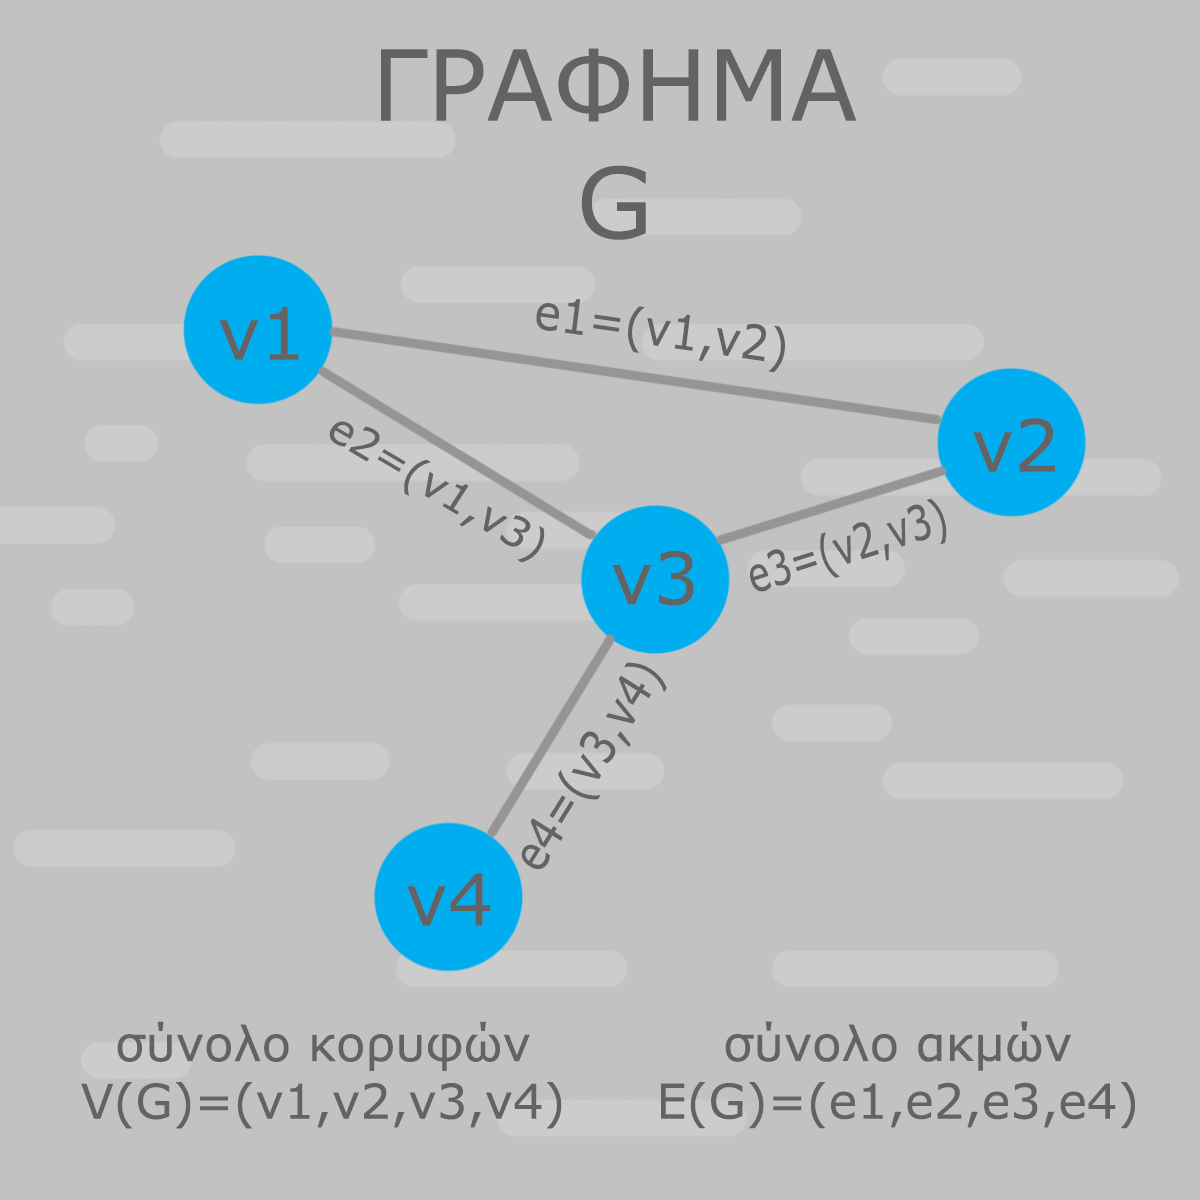
\includegraphics[scale=0.30]{2947_thesis/pictures/synola.png} 
    \caption{Σύνολα γραφήματος.}
    \label{7}
\end{figure}


\subsection{Αναπαράσταση γράφων}
Την κλασσική μορφή αναπαράστασης ενός γράφου την είδαμε ήδη παραπάνω, όπως φαίνεται στο σχήμα \ref{3}, όμως μια τέτοια αναπαράσταση δεν είναι καθόλου πρακτική σε προγραμματιστικό επίπεδο. Για αυτό αν θέλουμε να αναπαραστήσουμε γράφους σε έναν υπολογιστή χρησιμοποιούμε δομές δεδομένων. Οι δύο πιο βασικοί μέθοδοι αναπαράστασης γράφων σε υπολογιστές είναι οι πίνακες γειτνίασης (\lt{adjacency table}) και οι λίστες γειτνίασης (\lt{adjacency lists})\footnote{Αναπαράσταση γράφων, Παναγιώτα Φατούρου, Πανεπιστήμιο Κρήτης\\link: \url{https://www.csd.uoc.gr/~hy240/current/material/teacherClasses/Section10.pdf}}.

Πίνακα γειτνίασης (\lt{adjacency table}) ονομάζουμε ένα πίνακα μεγέθους $n\times n$, όπου $n$ ο αριθμός των κορυφών του γράφου. Κάθε κελί του πίνακα δείχνει την σχέση των αναγραφόμενων κορυφών. Σε ένα μη-κατευθυνόμενος γράφο το κελί $[i, j]$ παίρνει την τιμή 1 αν υπάρχει η ακμή $i \longleftrightarrow j$ και 0 αν δεν υπάρχει. 

Δηλαδή, έστω ο πίνακας γειτνίασης A του γράφου $G$:
\begin{center}
    $A[i, j] = 
    \begin{cases}
      1 & \text{αν $(i,j) \in E(G)$}\\
      0 & \text{αλλού}
    \end{cases}$
\end{center}
Είναι εύκολα αντιληπτό ότι ο πίνακας αυτός θα είναι συμμετρικός, δηλαδή ισούτε με τον ανάστροφό του, αφού η ακμή $i \longleftrightarrow j$ είναι ίδια με την ακμή $j \longleftrightarrow i$. Αντίστοιχα, σε έναν κατευθυνόμενο γράφο, το κελί $[i, j]$ παίρνει ομοίως τιμές 0 και 1 με την διαφορά ότι ο πίνακας δεν είναι συμμετρικός, οπότε η ακμή $i \rightarrow j \neq j \rightarrow i$. 

Οι πίνακες γειτνίασης μπορεί να έχουν και βάρη (\lt{weights}) που είναι μια επέκταση του απλού πίνακα γειτνίασης, σε αυτήν την περίπτωση, το έκαστο κελί ενός πίνακα, αντί για 1, περιέχει έναν αριθμό που ονομάζετε βάρος (\lt{weight}) και υποδηλώνει κάτι ανάλογα με την χρήση του. Σε έναν αλγόριθμο βελτιστοποίησης το βάρος μπορεί να υποδηλώνει την απόσταση της μιας κορυφής από την άλλη, την πιθανότητα επιλογής αυτής της διαδρομής, την επιρροή που δέχεται κάποια οντότητα σε επόμενο πιθανό πείραμα ή οποιοδήποτε άλλο κριτήριο που ανταποκρίνεται στον σκοπό του συγκεκριμένου αλγορίθμου\footnote{Πίνακες γειτνίασης, Παναγιώτα Φατούρου, Πανεπιστήμιο Κρήτης \\link: \url{https://www.csd.uoc.gr/~hy240/current/material/teacherClasses/Section10.pdf}} \cite{gkertsis2023thewria}.


Για παράδειγμα στο σχήμα \ref{7}, πρόκειται για έναν μη-κατευθυνόμενο γράφο χωρίς βάρη με 4 κορυφές, δηλαδή $n=4$ και με ακμές που φαίνονται στο σύνολο $E(G)$. Επομένως ο πίνακας γειτνίασης του διαμορφώνεται έτσι: 
$$
G_{n,n} = 
\begin{array}{c|c c c c}
   & v_{1} & v_{2} & v_{3} & v_{4} \\ \hline
   v_{1} & v_{1,1} & v_{1,2} & v_{1,3} & v_{1,4} \\
   v_{2} & v_{2,1} & v_{2,2} &   v_{2,3} & v_{2,4} \\
   v_{3} & v_{3,1} & v_{3,2} & v_{3,3} & v_{3,4} \\
   v_{4} & v_{4,1} & v_{4,2} & v_{4,3} & v_{4,4} 
\end{array}
$$
που αντικαθιστώντας 0-1 προκύπτει: 
$$
G_{4,4} = 
\begin{array}{c|c c c c}
   & v_{1} & v_{2} & v_{3} & v_{4} \\ \hline
   v_{1} & 0 & 1 & 1 & 0 \\
   v_{2} & 1 & 0 & 1 & 0 \\
   v_{3} & 1 & 1 & 0 & 1 \\
   v_{4} & 0 & 0 & 1 & 0 
\end{array}
$$
όπου 1 συμβολίζει ότι αυτές οι δύο κορυφές είναι γειτονικές έχοντας ακμή να τις ενώνει, ενώ 0 ότι δεν υπάρχει ακμή.

Λίστα γειτνίασης (\lt{adjacency list}) ονομάζουμε μια αναπαράσταση γράφων όπου για κάθε κορυφή διατηρείται μια λίστα των γειτόνων της. Σε περίπτωση κατευθυνόμενου γράφου μπορεί να υπάρχει ξεχωριστή λίστα για τους εξερχόμενους και τους εισερχόμενους γείτονες-κορυφές. Αυτή η αναπαράσταση αποκτά αξία σε γράφους με αραιή (\lt{sparse}) συνδεσιμότητα αφού γίνεται εξοικονόμηση μνήμης\footnote{Λίστες Γειτνίασης, Παναγιώτα Φατούρου, Πανεπιστήμιο Κρήτης \\link: \url{https://www.csd.uoc.gr/~hy240/current/material/teacherClasses/Section10.pdf}}.

Το πόσο μεγάλη θα είναι η λίστα εξαρτάται από τον αριθμό των κορυφών του γράφου. Κάθε στοιχείο στην λίστα συμβολίζει μία ακμή του γράφου. Στην περίπτωση ενός μη-κατευθυνόμενου γράφο, η λίστα γειτνίασης για κάθε κορυφή περιλαμβάνει τους γείτονές της, δηλαδή τις άλλες κορυφές με τις οποίες συνδέεται με μια ακμή. Αν υπάρχουν $n$ κορυφές στον γράφο, η λίστα γειτνίασης για κάθε κορυφή περιλαμβάνει μια λίστα με το πλήθος των γειτόνων της. Για παράδειγμα στο σχήμα \ref{7} που απεικονίζεται ένας μη-κατευθυνόμενος γράφος με 4 κορυφές, άρα $n=4$ και ακμές που φαίνονται στο σύνολο $E(G)$ του αντίστοιχου σχήματος, αν η αναπαράσταση γινόταν με λίστα γειτνίασης θα ήταν ως εξής: 
\begin{enumerate}
    \item $v_1: \{v_2, v_3\}$
    \item $v_2: \{v_1, v_3\}$
    \item $v_3: \{v_1, v_2, v_4\}$
    \item $v_4: \{v_3\}$
\end{enumerate}

Στην περίπτωση ενός κατευθυνόμενου γράφου, σε κάθε κορυφή θα υπάρχαν 2 λίστες, μία που εκφράζει τις προηγούμενες κορυφές και μία που εκφράζει τις ακόλουθες. Για παράδειγμα στο σχήμα \ref{6} η λίστα γειτνίασης θα αναπαριστόταν ως εξής: 
\begin{enumerate}
    \item Α: προηγούμενοι:$\{B, Γ\}$, ακόλουθοι:$\{B\}$
    \item Β: προηγούμενοι:$\{A, E\}$, ακόλουθοι:$\{A, E\}$
    \item Γ: προηγούμενοι:$\{E\}$, ακόλουθοι:$\{A, Z\}$
    \item Δ: προηγούμενοι:$\{Z\}$, ακόλουθοι:$\{E\}$
    \item Ε: προηγούμενοι:$\{Δ, Z\}$, ακόλουθοι:$\{B, Γ\}$
    \item Ζ: προηγούμενοι:$\{Γ\}$, ακόλουθοι:$\{Δ, E\}$
    
\end{enumerate}


Σε σχέση με τους πίνακες γειτνίασης, οι λίστες γειτνίασης επιτρέπουν την εύκολη πρό- σβαση στα δεδομένα του γράφου καθώς και τροποποίηση αυτών, δηλαδή η εισαγωγή και η διαγραφή μιας κορυφής μπορεί να γίνει με ευκολία. Επίσης σε αραιούς γράφους (δηλαδή γράφους με λίγες ακμές) απαιτούν λιγότερη μνήμη, ενώ σε πλήρη συνδεδεμένους γράφους περισσότερη. Αντίθετα, οι πίνακες γειτνίασης δεν επιτρέπουν εύκολη τροποποίηση στις κορυφές και τις σχέσεις μεταξύ τους, ούτε εύκολη εισαγωγή και διαγραφή, για παράδειγμα μία πιθανή εισαγωγή θα προκαλέσει αύξηση στο μέγεθος του πίνακα\footnote{Θετικά και Αρνητικά, Παναγιώτα Φατούρου, Πανεπιστήμιο Κρήτης \\link: \url{https://www.csd.uoc.gr/~hy240/current/material/teacherClasses/Section10.pdf}}. Όμως, το γεγονός ότι πολλές λειτουργίες μπορούν απλά και αποτελεσματικά να μοντελοποιηθούν τους κάνει ιδανικούς για χρήση στον αλγόριθμο μας. 


%Σειριακός Προγραμματισμός
\section{Αλγόριθμοι Βέλτιστης Διαδρομής}
Θα παρουσιαστούν ορισμένοι αλγόριθμοι που θα επιλέξω και θα γραφούν αναλογα υποπαράγραφοι για τον καθένα

%Παράλληλος Προγραμματισμός
\section{Αλγόριθμος Αποικίας Μυρμηγκιών}
Θα παρουσιαστεί αυτός ο αλγόριθμος
\subsection{συγκρίσεις}
Θα συγκριθούν οι αλγόριθμοι που αναλύθηκαν 
\subsection{Υλοποίησή μου Αλγόριθμου Αποικίας Μυρμηγκιών}
Θα γίνει αναφορά του κώδικα που θα γράψω σε \lt{python} και θα συγκριθεί με ήδη υπάρχοντες
\subsection{Εφαρμογές Αλγόριθμου Αποικίας Μυρμηγκιών}
Θα δωθούν  προβλήματα πραγματικού κόσμου που λύνει αυτός ο αλγόριθμος

οι αναφορές δεν έχουν δωθεί ακόμα


%%%%%%%%%%%%%%%%%%%%%%%%%%%%%%%%%%%%%%%%


% Βιβλιογραφία - Αναφορές

	%\bibliography{references}
        \begin{otherlanguage*}{english}
		\bibliography{biblio}
		\end{otherlanguage*}
	\bibliographystyle{plain}
	
% Παραρτήματα
	%\appendix
	\section*{Εγκατάσταση και εκτέλεση {\lt Anaconda} διανομής και {\lt jupyter notebook}}

Το anaconda είναι μια διανομή ανοιχτού κώδικα, στην οποία περιλαμβάνεται και το jupyter notebook για εκτέλεση κώδικα σε python, παράλληλα με άλλα χρήσιμα εργαλία. Κατεβάζουμε την διανομή από την ιστοσελίδα τους (\url{https://www.anaconda.com/download}) ανάλογα με το λειτουργικό που χρησιμοποιούμε, και το τρέχουμε. Κατεβάζουμε με τα default settings. Τρέχουμε το πρόγραμμα και θα μας ανοίξει το anaconda navigator με πολλά διαθέσιμα εργαλεία, θα υπάρχει και το jupyter notebook, το κατεβάζουμε και ανοιγουμε ένα new jupyter notebook. Θα μας ανοίξει ένα καινούργιο παράθυρο στο οποίο μπορούμε να γράψουμε κώδικα σε γλώσσα python. Εκεί εκτελούμε όλους τους αλγόριθμους που παρουσιάζονται σε αυτήν την εργασία.

\newpage 

	\include{end_sections/glossary}	
	\nocite{*}
	
	\appendix

%%%%%%%%%%%%%%%%%%%%%%%%%%%%%%%%%%%%%%%%%%%%%%%%%%%%
%\backmatter
% Ευρετήριο Όρων
%	\printindex
%	\cleardoublepage

\end{document}
